
\فصل{نوشتن برنامه Hello World با EFI}

در این قسمت برای شروع کار یک برنامه‌ی Hello World می‌نویسیم.

\قسمت{آماده کردن محیط برنامه نویسی EFI}

برای این قسمت ما از \لر{edk2} استفاده کرده‌ایم که می‌توانید آن را در این \href{https://github.com/tianocore/edk2}{لینک} مشاهده کنید. این ابزار یک سری کتابخانه برای نوشتن و ساختن برنامه‌ها و درایورهای \لر{EFI} است.

\قسمت{تحلیل کد}

کد این قسمت در \لر{HelloWorld.c} نوشته شده است. تابع \لر{UefiMain} تابعی است که در شروع برنامه اجرا می‌شود. در خط اول توسط تابع \لر{Print} رشته مورد نظر را چاپ می‌کنیم و دقت می‌کنیم که در \لر{UEFI} باید از رشته‌های عریض (کاراکترهای ۲ بایتی) استفاده شود.

\قسمت{اجرای کد}
برای اجرای کد با استفاده از \لر{QEMU} و \لر{OVMF} یک محیط \لر{EFI} بالا می‌آوریم تا برنامه را در آن اجرا کنیم. این کار با دادن \لر{OVMF} به عنوان آپشن \لر{bios} به \لر{QEMU} به سادگی قابل انجام است. این اجرا در \رجوع{fig:helloworld1} قابل مشاهده است.
\begin{figure}
	\centering
	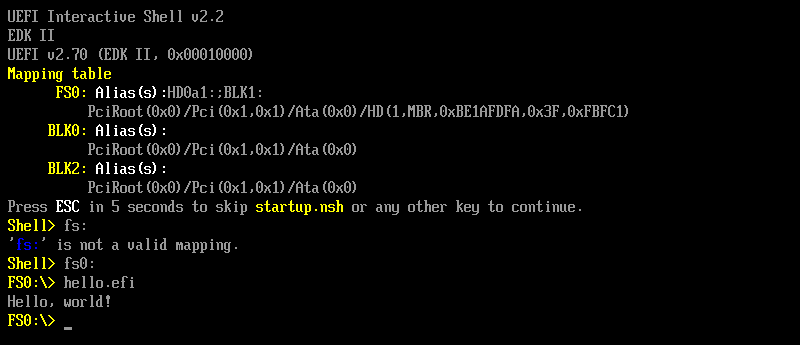
\includegraphics[width=0.7\linewidth]{figs/helloworld/helloworld1}
	\caption{اجرای برنامه‌ی \لر{hello.efi}}
	\label{fig:helloworld1}
\end{figure}
